\section{Propuesta Técnica}

\subsection{Título y Resumen}
El proyecto consiste en el análisis, diseño y desarrollo de una aplicación digital que facilite la organización del tiempo y la realización autónoma de actividades cotidianas principalmente a estudiantes con discapacidad intelectual, especialmente a aquellos que participan en el Programa de Transición a la Vida Adulta (PTVAL) del Colegio de Educación Especial Fundación Purísima Concepción de Granada. La aplicación permitirá consultar una agenda personalizada, visualizar las actividades programadas y acceder a instrucciones adaptadas a las necesidades de cada estudiante.

La solución incorporará distintos perfiles de usuario y opciones de personalización de la interfaz, como el tamaño y tipo de letra, los colores y los elementos visuales empleados. También permitirá gestionar actividades, consultar sus detalles y registrar su inicio, progreso y finalización. De esta forma, se pretende facilitar la comprensión de las tareas, favorecer la autonomía del alumnado y mejorar la coordinación entre estudiantes, tutores y profesores. El desarrollo se realizará siguiendo la metodología Scrum, mediante tres iteraciones, y prestando especial atención a la accesibilidad, la usabilidad y la protección de los datos personales.

\subsection{Duración en Meses}
El proyecto se desarrollará desde el 25 de septiembre de 2026 hasta el 21 de diciembre de 2026. Su duración total será de aproximadamente tres meses, incluyendo la preparación inicial, las tres iteraciones de desarrollo y las actividades de cierre y documentación final.

\subsection{Tipo de Caso de Negocio}
El proyecto responde principalmente a una demanda de un cliente, el Colegio de Educación Especial Fundación Purísima Concepción de Granada, que necesita una herramienta digital para facilitar la organización del tiempo y promover la autonomía de estudiantes con discapacidad intelectual.

La iniciativa también responde a una necesidad de mejora de accesibilidad, ya que las soluciones existentes no siempre se adaptan suficientemente a las capacidades cognitivas, preferencias y necesidades de cada estudiante. Por tanto, se propone desarrollar una aplicación que facilite la personalización de las agendas y simplifique la gestión de actividades por parte de los tutores y profesores.

\subsection{Objetivos}

\subsubsection{Objetivo General}
Diseñar, desarrollar y verificar una aplicación web accesible y personalizable que facilite la planificación y realización de actividades escolares y personales de estudiantes con discapacidad intelectual, permitiendo su gestión y seguimiento por parte de los propios estudiantes, sus tutores y los profesores autorizados.

\subsubsection{Objetivos Específicos}
\definecolor{verdeTag}{HTML}{2E7D32}
\definecolor{amarilloTag}{HTML}{E65100}
\definecolor{grisTag}{HTML}{616161}

\paragraph{Requisitos Funcionales (RF)}
Definen las funcionalidades que deberá proporcionar la aplicación. A continuación se detalla su alcance y nivel de cobertura en el proyecto:

\begin{xltabular}{\textwidth}{|p{2.2cm}|X|p{2.8cm}|}
\hline
\rowcolor{azulPastelApagado}
\textbf{Código} & \textbf{Descripción del Requisito Funcional} & \textbf{Estado / Alcance} \\ \hline
\endhead

\hline
\endfoot

\rowcolors{2}{azulclaro}{white}
\textbf{RF1} & Implementar un sistema de inicio de sesión que permita a cada usuario acceder a las funcionalidades correspondientes a su perfil. & \cellcolor{verdeApagado}\textbf{Incluido} \\ \hline
\textbf{RF2} & Permitir al profesor consultar los estudiantes que tiene asignados y seleccionar uno para acceder a su información. & \cellcolor{verdeApagado}\textbf{Incluido} \\ \hline
\textbf{RF3} & Permitir al administrador gestionar cuentas de estudiantes, profesores y tutores. & \cellcolor{verdeApagado}\textbf{Incluido} \\ \hline
\textbf{RF3.1} & --- Crear cuentas de estudiantes, profesores y tutores. & \cellcolor{verdeApagado}\textbf{Incluido} \\ \hline
\textbf{RF3.2} & --- Eliminar cuentas de estudiantes, profesores y tutores. & \cellcolor{verdeApagado}\textbf{Incluido} \\ \hline
\textbf{RF3.3} & --- Establecer relaciones entre estudiantes, profesores y tutores legales. & \cellcolor{verdeApagado}\textbf{Incluido} \\ \hline
\textbf{RF3.4} & --- Editar cuentas de estudiantes, profesores y tutores. & \cellcolor{verdeApagado}\textbf{Incluido} \\ \hline
\textbf{RF5} & Permitir a la familia consultar el perfil de un estudiante. & \cellcolor{verdeApagado}\textbf{Incluido} \\ \hline
\textbf{RF6} & Permitir a la Familia consultar y editar sus preferencias de configuración. & \cellcolor{verdeApagado}\textbf{Incluido} \\ \hline
\textbf{RF7} & Permitir al estudiante sus preferencias de configuración. & \cellcolor{verdeApagado}\textbf{Incluido} \\ \hline
\textbf{RF7.1} & --- Preferencias de texto (Tamaño, pictogramas, contraste). & \cellcolor{verdeApagado}\textbf{Incluido} \\ \hline
\textbf{RF7.1.1} & ------ Mostrar pictogramas en lugar de texto plano. & \cellcolor{verdeApagado}\textbf{Incluido} \\ \hline
\textbf{RF7.1.2} & ------ Permitir inputs de texto mediante voz. & \textit{Opcional} \\ \hline
\textbf{RF7.1.3} & ------ Preferencias de contraste. & \cellcolor{verdeApagado}\textbf{Incluido} \\ \hline
\textbf{RF7.1.4} & ------ Preferencias de tamaño de texto. & \cellcolor{verdeApagado}\textbf{Incluido} \\ \hline
\textbf{RF7.1.5} & ------ Preferencias respecto al tiempo. & \cellcolor{verdeApagado}\textbf{Incluido} \\ \hline
\textbf{RF7.2} & --- Preferencias de colores de la aplicación. & \cellcolor{verdeApagado}\textbf{Incluido} \\ \hline
\textbf{RF8} & Permitir al estudiante cambiar su imagen de perfil de usuario. & \cellcolor{verdeApagado}\textbf{Incluido} \\ \hline
\textbf{RF9} & Mostrar al estudiante las actividades programadas para un día seleccionado. & \cellcolor{verdeApagado}\textbf{Incluido} \\ \hline
\textbf{RF10} & Mostrar al estudiante consultar las actividades de la semana. & \cellcolor{verdeApagado}\textbf{Incluido} \\ \hline
\textbf{RF11} & Consultar detalles de una actividad (imagen, descripción, horario, instrucciones). & \cellcolor{verdeApagado}\textbf{Incluido} \\ \hline
\textbf{RF11.1} & --- Permitir al profesor acceder a la lista de estudiantes participantes. & \cellcolor{verdeApagado}\textbf{Incluido} \\ \hline
\textbf{RF12} & Crear actividades personales y escolares indicando detalles completos. & \cellcolor{verdeApagado}\textbf{Incluido} \\ \hline
\textbf{RF13} & Editar y cancelar actividades propias actualizando las agendas afectadas. & \cellcolor{verdeApagado}\textbf{Incluido} \\ \hline
\textbf{RF14} & Permitir a la familia editar/cancelar actividades creadas por el estudiante. & \cellcolor{verdeApagado}\textbf{Incluido} \\ \hline
\textbf{RF15} & Permitir al profesor asignar actividades a grupos o estudiantes concretos. & \cellcolor{verdeApagado}\textbf{Incluido} \\ \hline
\textbf{RF16} & Permitir al estudiante confirmar el inicio y la finalización de una actividad. & \cellcolor{verdeApagado}\textbf{Incluido} \\ \hline
\textbf{RF17} & Marcar individualmente los pasos de una actividad completada en secuencia. & \cellcolor{verdeApagado}\textbf{Incluido} \\ \hline
\textbf{RF18} & Configurar la visualización de un reloj/indicador de tiempo en actividades. & \cellcolor{verdeApagado}\textbf{Incluido} \\ \hline
\textbf{RF19} & Permitir al estudiante recibir avisos del comienzo de actividades. & \cellcolor{verdeApagado}\textbf{Incluido} \\ \hline
\textbf{RF20} & Incorporar un canal de comunicación accesible entre estudiante y tutores. & No incluido \\ \hline
\textbf{RF21} & Proponer actividades optativas automáticas si una tarea se cancela. & No incluido \\ \hline
\textbf{RF22} & Valorar actividades realizadas para personalizar futuras sugerencias. & No incluido \\ \hline
\textbf{RF23} & Avisar al estudiante cuando una actividad asignada sea cancelada. & \textit{Opcional} \\ \hline
\textbf{RF24} & Bloqueo de inicio de sesión tras 5 intentos fallidos en 2 minutos. & \cellcolor{verdeApagado}\textbf{Incluido} \\ \hline
\end{xltabular}

\vspace{0.6cm}

\paragraph{Requisitos No Funcionales (RNF)}
Definen las condiciones de calidad, accesibilidad, seguridad y funcionamiento que deberá cumplir la aplicación.

\begin{table}[H]
\centering
\rowcolors{1}{white}{white}
\begin{tabularx}{\textwidth}{|p{2.2cm}|X|}
\hline
\rowcolor{azulPastelApagado}
\textbf{Código} & \textbf{Criterios de Calidad y Usabilidad} \\ \hline
\rowcolor{azulclaro}
\textbf{RNF1} & Diseñar una interfaz sencilla, consistente y comprensible, reduciendo la cantidad de información y opciones mostradas simultáneamente al estudiante. \\ \hline
\textbf{RNF2} & Permitir adaptar la presentación de la aplicación a las necesidades individuales mediante las opciones de personalización disponibles. \\ \hline
\rowcolor{azulclaro}
\textbf{RNF3} & Utilizar textos claros y concisos, instrucciones breves, iconos comprensibles y apoyos visuales adecuados para facilitar la comprensión de las actividades. \\ \hline
\textbf{RNF4} & Facilitar la interacción mediante controles suficientemente grandes, una disposición clara de los elementos y una navegación sencilla, teniendo en cuenta las necesidades de movilidad de los usuarios. \\ \hline
\rowcolor{azulclaro}
\textbf{RNF5} & Garantizar que las funcionalidades principales puedan utilizarse desde los navegadores y dispositivos compatibles definidos para el proyecto. \\ \hline
\textbf{RNF6} & Proteger el acceso a la información mediante autenticación y comprobación de permisos según el perfil del usuario. \\ \hline
\rowcolor{azulclaro}
\textbf{RNF7} & Garantizar que los usuarios solo puedan consultar o modificar la información para la que tengan autorización. \\ \hline
\textbf{RNF8} & Aplicar medidas de protección de datos personales, limitando la información recogida a la necesaria y cumpliendo la normativa aplicable. \\ \hline
\rowcolor{azulclaro}
\textbf{RNF9} & Diseñar e implementar paletas de colores coherentes para mostrar en la aplicación. \\ \hline
\textbf{RNF10} & Diseñar una página de login accesible. \\ \hline
\end{tabularx}
\end{table}

\vspace{0.6cm}

\paragraph{Requisitos de Implementación (RI)}
Definen las tecnologías, herramientas y condiciones técnicas previstas para desarrollar y ejecutar la solución.

\begin{table}[H]
\centering
\rowcolors{1}{white}{white}
\begin{tabularx}{\textwidth}{|p{2.2cm}|X|}
\hline
\rowcolor{azulPastelApagado}
\textbf{Código} & \textbf{Especificación Técnica / Restricción de Dominio} \\ \hline
\rowcolor{azulclaro}
\textbf{RI1} & Respecto de los usuarios se debe almacenar: correo, nombre de usuario, nombre real, fecha de nacimiento. \\ \hline
\textbf{RI2} & Cuando una cuenta es dada de baja, sus datos permanecen almacenados al menos 4 años. \\ \hline
\rowcolor{azulclaro}
\textbf{RI3} & Los usuarios pertenecen a una de las siguientes categorías: Estudiante, Profesor, Familia o Administrador. \\ \hline
\textbf{RI4} & Los usuarios deben poder seleccionar sus preferencias de personalización y estas deben permanecer entre sesión y sesión. \\ \hline
\rowcolor{azulclaro}
\textbf{RI5} & Las actividades deben tener una descripción que puede componerse de texto, imágenes o videos. \\ \hline
\textbf{RI6} & Las actividades pueden contener varios pasos personalizables y verificables individualmente. \\ \hline
\rowcolor{azulclaro}
\textbf{RI7} & Las actividades deben almacenar su estado de “sin empezar/comenzada/terminada”. \\ \hline
\textbf{RI8} & Los estudiantes pueden tener actividades asignadas en una fecha concreta con una hora de inicio y fin dadas. \\ \hline
\rowcolor{azulclaro}
\textbf{RI9} & Los profesores y la familia pueden crear actividades para asignarlas a los estudiantes. \\ \hline
\textbf{RI10} & Los estudiantes podrán estar relacionados con profesores y familia de forma específica. \\ \hline
\rowcolor{azulclaro}
\textbf{RI11} & Los estudiantes pueden pertenecer a grupos de clase. \\ \hline
\textbf{RI12} & Uno o varios profesores pueden enviar tareas a un grupo de estudiantes. \\ \hline
\rowcolor{azulclaro}
\textbf{RI13} & Las contraseñas deben ser cifradas a la hora de almacenarlas. \\ \hline
\end{tabularx}
\end{table}

\subsection{Antecedentes del Equipo de Trabajo}
El equipo está formado por seis estudiantes de último año con formación en Ingeniería Informática, los cuales contamos con conocimientos en distintas áreas, lenguajes de programación y herramientas de desarrollo que nos permiten afrontar el análisis, diseño, programación y pruebas del sistema exigidas.

Dado que no todos tenemos la misma experiencia previa en desarrollo web, reservaremos un tiempo inicial para formarnos e igualar el nivel técnico del grupo. Además, aunque tenemos una base sólida en distintas áreas de trabajo, esta es nuestra primera experiencia trabajando en un equipo de desarrollo con un enfoque similar al profesional. Por ello, nos organizaremos bien a la hora de coordinarnos, repartirnos las tareas, gestionar el control de versiones y revisar el trabajo, asegurando así una buena colaboración y un resultado de calidad.

\subsection{Justificación: Revisión de Soluciones Relacionadas con la Temática Comparativa}
Existen aplicaciones y recursos que permiten organizar actividades mediante agendas visuales, imágenes y pictogramas. Algunas de ellas son las siguientes:

\begin{itemize}
    \item \textbf{PictogramAgenda:} Permite crear secuencias ordenadas de pictogramas, destacar la actividad actual, marcar tareas realizadas y utilizar sonido y temporizadores.
    \item \textbf{Día a Día:} Ofrece un diario visual para registrar y anticipar actividades mediante imágenes, fotografías, vídeos, sonidos y textos, con opciones de personalización.
\end{itemize}
\begin{figure}[htbp]
    \centering
    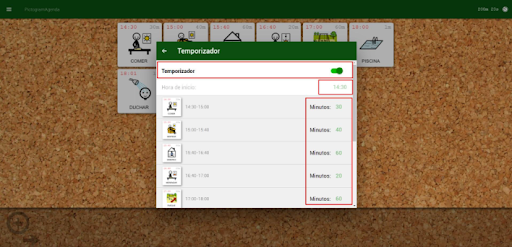
\includegraphics[width=0.8\textwidth]{img/pictograma_agenda.png}
    \caption{Foto de PictogramAgenda}
    \label{fig:pictogram_agenda}
\end{figure}
\begin{figure}[htbp]
    \centering
    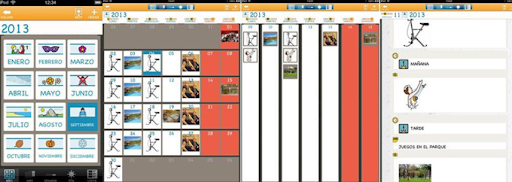
\includegraphics[width=0.8\textwidth]{img/dia_a_dia.png}
    \caption{Foto de Dia a Dia Agenda.}
    \label{fig:dia_a_dia_agenda}
\end{figure}

A continuación, vamos a realizar una comparativa de las agendas que hay en el mercado con la propuesta que se nos ofrece, para ver en qué se diferencia y qué aspectos añaden valor a nuestra agenda con respecto a otras opciones propuestas en el mercado.

\begin{table}[H]
\centering
\rowcolors{2}{azulclaro}{white}
\begin{tabularx}{\textwidth}{X p{2.8cm} p{2.8cm} p{3.2cm}}
\toprule
\rowcolor{azulPastelApagado}
\textbf{Característica} & \textbf{PictogramAgenda} & \textbf{Día a Día} & \textbf{Agenda Doble} \\
\midrule
Organización visual de actividades & Sí & Sí & Sí \\
Imágenes y pictogramas & Sí & Sí & Sí \\
Personalización visual & Algunas opciones & Sí & Orientada a cada perfil \\
Gestión de perfiles de estudiante y tutor & No es su función principal & No es su función principal & Sí \\
Asignación y seguimiento de actividades escolares & Limitado al uso de la agenda visual & No es su función principal & Sí \\
Gestión de actividades personales & Sí, mediante secuencias & Sí, mediante diario visual & Sí \\
\bottomrule
\end{tabularx}
\caption{Comparativa de soluciones existentes frente a Agenda Doble.}
\end{table}

En definitiva, aunque ya existen herramientas que ofrecen buenas funciones para organizar actividades visualmente, nuestro objetivo es unificar la gestión de usuarios, perfiles personalizados y un control completo de las tareas escolares y personales en nuestra aplicación, siendo lo más personalizable posible y adaptado al día a día del estudiante.

\subsection{Descripción y Esquema de Solución}
\textit{(CREO QUE ESTA ES LA PROPUESTA DE SOLUCIÓN)}

La solución consistirá en una aplicación web accesible y adaptable a distintos dispositivos, destinada principalmente a estudiantes del PTVAL y a las personas autorizadas que les acompañan. La aplicación organizará sus funcionalidades según el perfil del usuario, evitando mostrar opciones innecesarias y facilitando una interacción sencilla.

El estudiante podrá consultar su agenda, visualizar la información de las actividades, acceder a instrucciones adaptadas, marcar los pasos realizados y confirmar el inicio y la finalización de las tareas. Según la configuración disponible, podrá consultar actividades de los próximos días, personalizar sus preferencias y crear actividades personales.

Los tutores y profesores podrán gestionar las actividades de los estudiantes que tengan asignados, consultar sus perfiles y realizar un seguimiento de su progreso. El administrador se encargará de gestionar las cuentas y las relaciones entre usuarios. Las funcionalidades se implementarán de forma progresiva, atendiendo a la prioridad de las historias de usuario y al tiempo disponible.

\subsubsection{Tecnologías Previstas}
\begin{itemize}
    \item \textbf{HTML:} estructura de las páginas.
    \item \textbf{CSS:} presentación visual y adaptación de la interfaz a diferentes necesidades.
    \item \textbf{JavaScript:} interacciones y funcionalidades del lado del cliente.
    \item \textbf{PHP:} lógica del servidor, validación de peticiones y comunicación con la base de datos.
    \item \textbf{MySQL:} almacenamiento de usuarios, perfiles, actividades y registros de seguimiento.
    \item \textbf{Docker:} ejecución de los servicios en contenedores.
    \item \textbf{Git y GitHub:} control de versiones y trabajo compartido.
\end{itemize}

\subsubsection{Arquitectura Propuesta}
La aplicación seguirá una arquitectura web cliente-servidor organizada en tres niveles: interfaz de usuario, lógica de aplicación y almacenamiento de datos.

\begin{enumerate}
    \item \textbf{Presentación:} el navegador mostrará la interfaz desarrollada con HTML, CSS y JavaScript.
    \item \textbf{Lógica de aplicación:} el servidor PHP gestionará la autenticación, los permisos, las operaciones sobre las actividades y las solicitudes de los usuarios.
    \item \textbf{Persistencia:} MySQL almacenará la información necesaria para el funcionamiento del sistema.
    \item \textbf{Despliegue:} Docker permitirá configurar y ejecutar los servicios necesarios de forma organizada.
\end{enumerate}

\paragraph{Esquema general:}
Usuario $\rightarrow$ Interfaz web (HTML, CSS y JavaScript) $\rightarrow$ Servidor PHP $\rightarrow$ Base de datos MySQL

\vspace{0.3cm}
Docker facilitará la ejecución de los componentes y GitHub permitirá mantener el código y su historial de cambios.

La aplicación deberá diseñarse teniendo en cuenta la accesibilidad cognitiva, visual y motora, así como la protección de los datos personales. Se priorizarán las instrucciones claras, los elementos visuales comprensibles, los controles fáciles de utilizar y la adaptación de la interfaz a cada perfil. La solución definitiva se concretará a partir de los requisitos acordados con el cliente y de las pruebas realizadas durante el desarrollo.

\subsection{Actividades a Realizar}
Las actividades se organizan provisionalmente en función de los objetivos específicos del proyecto. Su distribución definitiva se ajustará a la planificación acordada por el equipo.

\begin{table}[H]
\centering
\rowcolors{2}{azulclaro}{white}
\begin{tabularx}{\textwidth}{p{4.5cm} p{3.2cm} X}
\toprule
\rowcolor{azulPastelApagado}
\textbf{Actividad} & \textbf{Objetivos} & \textbf{Resultado esperado} \\
\midrule
A1. Análisis de requisitos y necesidades del cliente & 1, 2 & Especificación de requisitos e historias de usuario. \\
A2. Diseño de la interfaz y de la arquitectura & 2, 8 & Prototipos, diseño de la base de datos y arquitectura del sistema. \\
A3. Implementación de usuarios y perfiles & 4, 7 & Gestión de cuentas, permisos y preferencias. \\
A4. Desarrollo de la agenda y las actividades & 3, 4, 5, 6 & Consulta y gestión de actividades personales y escolares. \\
A5. Implementación de la personalización y accesibilidad & 2, 5, 8 & Interfaz adaptada a las necesidades de los usuarios. \\
A6. Pruebas y evaluación de calidad & 8, 9 & Registro de pruebas, incidencias y correcciones. \\
A7. Gestión y documentación del proyecto & 10 & Documentación actualizada, seguimiento y entregas. \\
\bottomrule
\end{tabularx}
\caption{Matriz de actividades, objetivos y resultados esperados.}
\end{table}

\subsection{Cronograma}

El proyecto seguirá una planificación basada en una fase inicial y tres iteraciones de desarrollo. Las fechas siguientes corresponden a la planificación proporcionada por el equipo.

\begin{table}[H]
\centering
\rowcolors{2}{azulclaro}{white}
\begin{tabularx}{\textwidth}{p{3cm} p{3cm} p{3cm} X}
\toprule
\rowcolor{azulPastelApagado}
\textbf{Fase} & \textbf{Inicio} & \textbf{Entrega prevista} & \textbf{Principales resultados} \\
\midrule
Iteración 0 & Fase inicial & 21-22 oct 2026 & Manual de coordinación, propuesta técnica y documentación inicial. \\
Iteración 1 & 22-23 oct 2026 & 11-12 nov 2026 & Primer incremento funcional y presentación de la iteración. \\
Iteración 2 & 12-13 nov 2026 & 2-3 dic 2026 & Segundo incremento, pruebas y presentación de resultados. \\
Iteración 3 & 3-4 dic 2026 & 21 dic 2026 & Incremento final previsto, pruebas y documentación asociada. \\
Cierre del proyecto & Tras iteración 3 & 6 feb 2027 & Revisión final, documentación pendiente y entrega definitiva. \\
\bottomrule
\end{tabularx}
\caption{Planificación y cronograma por fases e iteraciones.}
\end{table}

\subsection{Implicación de los Participantes}
\begin{itemize}
    \item \textbf{Equipo de desarrollo:} todos los integrantes participarán en el análisis, diseño, implementación, pruebas y documentación, según el reparto de tareas.
    \item \textbf{Coordinadores de cada iteración:} organizarán el trabajo, revisarán el avance y facilitarán la resolución de bloqueos.
    \item \textbf{Gestor de calidad:} supervisará las comprobaciones y el registro de incidencias.
    \item \textbf{Gestor de usabilidad y accesibilidad:} revisará la adecuación de la interfaz y las funcionalidades a las necesidades del alumnado.
    \item \textbf{Cliente y profesorado:} aportarán información sobre las necesidades, revisarán los avances y ayudarán a validar los requisitos.
\end{itemize}

La distribución concreta de funcionalidades y entregables por iteración se establecerá en el Product Backlog y en la planificación de cada iteración. Las fechas y los hitos intermedios deberán actualizarse si el profesorado establece otras condiciones.

\subsection{Cauces de Seguimiento}
El seguimiento del proyecto se realizará mediante reuniones periódicas con el profesorado o con el cliente. La comunicación formal con el mismo se realizará principalmente mediante correo electrónico para concertar reuniones mínimo una vez por iteración, donde se revisarán los avances, resolveremos dudas y validaremos las decisiones relacionadas con los requisitos.

Después de cada reunión se elaborarán actas en las que se recogerán los temas tratados, los acuerdos alcanzados y las cuestiones pendientes. Si el cliente solicita cambios, se analizará su prioridad, el esfuerzo necesario y su impacto sobre la planificación antes de incorporarlos al proyecto.

Para el seguimiento interno, se utilizará Jira, donde se registrarán las tareas, sus responsables y su estado. GitHub permitirá consultar la evolución del código y la documentación compartida. Además, el equipo mantendrá una comunicación continua mediante Discord y/o WhatsApp para resolver dudas y comunicar incidencias.

Al finalizar cada iteración se revisará el incremento desarrollado, se comprobará el cumplimiento de los objetivos previstos y se identificarán las mejoras necesarias para la siguiente fase.

\subsection{Valor Añadido}


Además de las funcionalidades básicas descritas en el pliego, la aplicación pretende aportar los siguientes elementos de valor añadido:

\begin{itemize}
    \item \textbf{Personalización centrada en el usuario:} adaptación de los elementos visuales y de la presentación de la agenda según las necesidades de cada estudiante.
    \item \textbf{Integración de actividades escolares y personales:} posibilidad de reunir en una misma herramienta las tareas asignadas en el centro y las actividades cotidianas.
    \item \textbf{Seguimiento del progreso:} consulta del estado de las actividades para facilitar el acompañamiento educativo.
    \item \textbf{Diseño modular:} organización de las funcionalidades por perfiles para facilitar su adaptación a las necesidades del centro.
    \item \textbf{Accesibilidad como criterio transversal:} consideración de las necesidades cognitivas, visuales y motoras desde el análisis hasta las pruebas finales.
    \item \textbf{Posible reutilización fuera del centro:} diseño de una herramienta que también pueda utilizarse como agenda personal por otros usuarios.
\end{itemize}

Las funcionalidades adicionales, como el chat accesible, las sugerencias de actividades alternativas o la valoración de tareas, se considerarán mejoras potenciales sujetas a la prioridad acordada y a la capacidad de desarrollo del equipo.

\subsection{Beneficios y Beneficiarios}

\subsubsection{Beneficiarios Directos}
\begin{itemize}
    \item \textbf{Estudiantes del PTVAL con discapacidad intelectual:} podrán consultar sus actividades de forma estructurada y adaptada a sus necesidades, favoreciendo su autonomía y participación en las tareas cotidianas.
    \item \textbf{Profesores y tutores del centro:} dispondrán de una herramienta para organizar actividades, asignarlas y consultar su estado.
    \item \textbf{Tutores legales y familiares:} podrán colaborar en la planificación de las actividades personales de los estudiantes que tengan asignados, dentro de los permisos establecidos.
\end{itemize}

\subsubsection{Beneficiarios Indirectos}
\begin{itemize}
    \item \textbf{Colegio de Educación Especial Fundación Purísima Concepción de Granada:} podrá disponer de una herramienta adaptada a sus necesidades educativas y organizativas.
    \item \textbf{Otros usuarios con necesidades de organización o accesibilidad:} podrán beneficiarse de las funciones de agenda y personalización, siempre que la solución final se adapte a sus necesidades.
\end{itemize}

\subsubsection{Beneficios Esperados}
El proyecto pretende favorecer la autonomía de los estudiantes, facilitar la comprensión de las actividades, reducir la complejidad de la planificación para los tutores y mejorar la coordinación entre el entorno educativo y familiar. Asimismo, permitirá al equipo aplicar conocimientos de ingeniería informática y gestión de proyectos en un contexto real de aprendizaje-servicio.

En cuanto a la propiedad intelectual, los productos y documentos resultantes serán de autoría compartida entre el equipo de trabajo y los peticionarios, de acuerdo con lo establecido en el pliego técnico.